%\title{Cdiscount Midterm Project Report}
\documentclass[10pt,twocolumn,letterpaper]{article}

\usepackage{cvpr}
\usepackage{times}
\usepackage{epsfig}
\usepackage{graphicx}
\usepackage{amsmath}
\usepackage{amssymb}
\usepackage{subcaption}

% Include other packages here, before hyperref.

% If you comment hyperref and then uncomment it, you should delete
% egpaper.aux before re-running latex.  (Or just hit 'q' on the first latex
% run, let it finish, and you should be clear).
\usepackage[pagebackref=true,breaklinks=true,letterpaper=true,colorlinks,bookmarks=false]{hyperref}

\cvprfinalcopy % *** Uncomment this line for the final submission

\def\cvprPaperID{****} % *** Enter the CVPR Paper ID here
\def\httilde{\mbox{\tt\raisebox{-.5ex}{\symbol{126}}}}

% Pages are numbered in submission mode, and unnumbered in camera-ready
\ifcvprfinal\pagestyle{empty}\fi
\begin{document}

%%%%%%%%% TITLE
\title{Cdiscount Midterm Project Report}

\author{Cagri Kaymak\\
Michigan State University \\
{\tt\small kaymakme@msu.edu}
% For a paper whose authors are all at the same institution,
% omit the following lines up until the closing ``}''.
% Additional authors and addresses can be added with ``\and'',
% just like the second author.
% To save space, use either the email address or home page, not both
\and
Matthew Andres Moreno\\
Michigan State University\\
{\tt\small mmore500@msu.edu}
\and
Ian Whalen\\
Michigan State University \\
{\tt\small whalenia@msu.edu}
}


\maketitle
%\thispagestyle{empty}

%%%%%%%%% ABSTRACT
\begin{abstract}
Online European retailer Cdiscount maintains an online catalog of 30 million products.
Cdiscount could achieve greater efficiency in managing its catalog of products by automating the product classificiation process. 
Cdiscount organizes its products into more than 5,000 categories, posing an extreme multi-category classification scheme problem.
We aim to develop an approach that leverages data made available by the retailer to allow for accurate, automated cataloging of products based on their images.
We will use existing convolutional neural network techniques (CNN) to classify images while exploiting the hierarchical nature of the Cdiscount categorization scheme to reduce the complexity of the problem.
\end{abstract}

%%%%%%%%% BODY TEXT
\section{Problem Description}
\begin{figure}
    \centering
    \begin{subfigure}[t]{0.33\columnwidth}
        \centering
        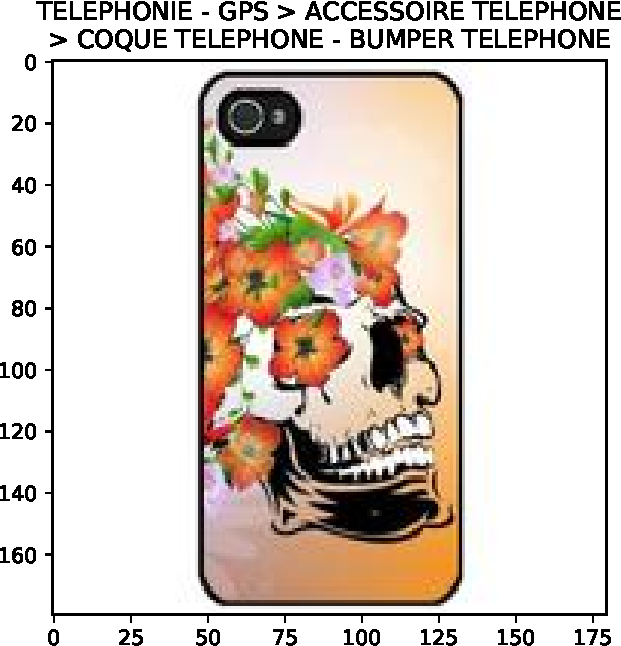
\includegraphics[width=\textwidth]{img/img-0-0}
        \caption{}
    \end{subfigure}%
    ~ 
    \begin{subfigure}[t]{0.33\columnwidth}
        \centering
        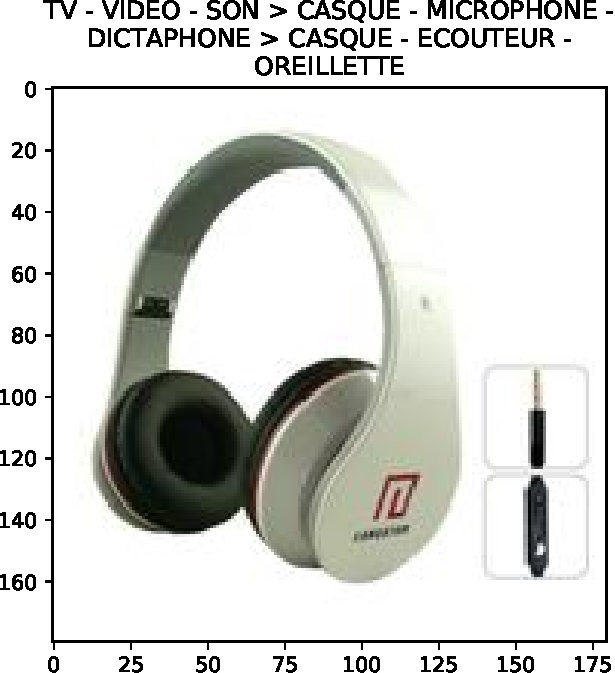
\includegraphics[width=\textwidth]{img/img-12-0}
        \caption{}
    \end{subfigure}%
    ~ 
    \begin{subfigure}[t]{0.33\columnwidth}
        \centering
        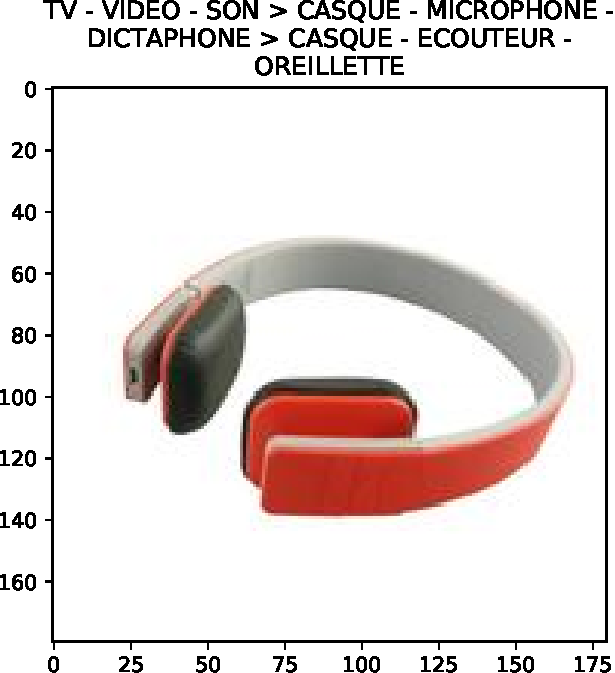
\includegraphics[width=\textwidth]{img/img-12-1}
        \caption{}
    \end{subfigure}
	\caption{
Images (a), (b), and (c) are three example training examples.
Image (a) is from a top level category different from images (b) and (c) (and therefore from different second and third categories, as well).
Images (b) and (c) are of the same product, and therefore from the same first, second ,and third level categories.
Only some products, not all, have more than one associated image.
}
	\label{fig:example-images}
\end{figure}

Cdiscount is one of France's largest e-commerce companies, selling large items such as trampolines, to small items like TVs.
As the company grows, so to does the number of different products they offer.
In the past 2 years alone, they have added over 20 million new products to their wares\cite{cDiscountKaggle}. 
Ensuring that each and every product is classified correctly is a challenging task.
Currently, Cdiscount uses machine learning text classification methods to categorize their wares.
To improve the accuracy of their classification methods, they would like to begin using images, rather than text, to categorize products.
The data set provided has over 15 million images ranging over 5,000 categories, and each image has 3 different levels of categorization, making this a challenging multi-classification problem.
Figure \ref{fig:example-images} shows example images from the Cdiscount dataset. 

\section{Data}

\begin{figure}

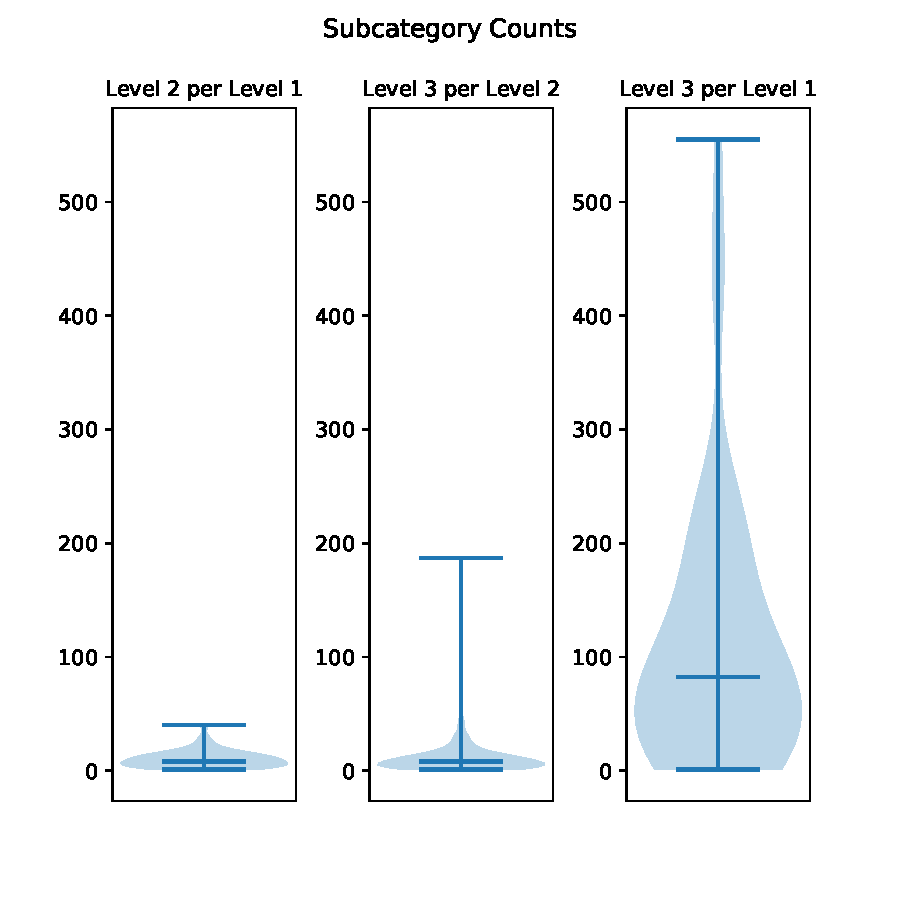
\includegraphics[width=\columnwidth]{img/catcount}
\caption{
This violin plot compares hierarchical category branching in the Cdiscount dataset.
The leftmost subplot presents the distribution of the number of second level subcategories in each top-level category.
The middle subplot presents the distribution of the number of third (bottom) level subcategories in each second level category.
The rightmost subplot presents the distribution of the number of bottom level subcategories in each first level category.
Going from first to second level and second to third level, categories branch by a median factor of approximately 10. 
From first to third level, categories branch by a median factor of approximately 100.
All three branching factor distributions have long right tails.
For example, going from second to third level, some categories are observed to branch by a factor of more than 150.
In all three subplots, horizontal bars mark the 0, 50, and 100th percentile counts.
}
\label{fig:catcount}

\end{figure}
\begin{figure}
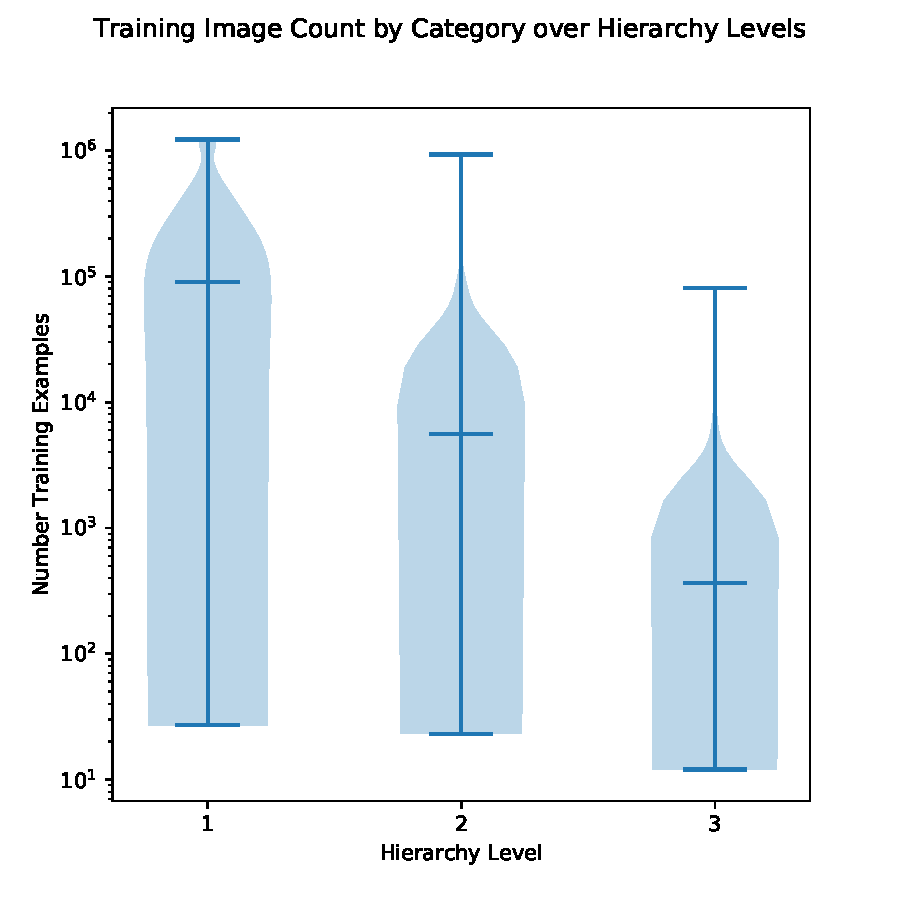
\includegraphics[width=\columnwidth]{img/datacount}
\caption{
This violin plot compares the number of training examples available for first (top) level categorizations, second level categorizations, and third (bottom) level categorizations.
As would be expected, the median training data count is highest for first level categories and lowest for third level categories.
On all three hierarchical levels, training data is distributed unevenly between categories.
For example, although the median top level category has approximately $10^5$ training examples, some have fewer than 100.
In all three subplots, horizontal bars mark the 0, 50, and 100th percentile counts.
}
\label{fig:datacount}
\end{figure}

Cdiscount has made an extensive dataset available through the data science platform Kaggle.
This dataset includes the full hierarchical categorization scheme used by Cdiscount and a listing of over 9 million products.
Each product has a unique ID, the ID of the category it falls in, and one to four images of that product.
The dataset comes divided into training and testing datasets, with the training set describing approximately 7 million products and the testing set describing approximately 2 million products.

Figure \ref{fig:catcount} shows the distribution of category-to subcategory branching.
Figure \ref{fig:datacount} shows the distribution of availability of training data over all categories in each hierarchy level.
As described in the figures, the categorical branching factors and data availabilities vary widely across the dataset.
These irregularities make the Cdiscount challenge more difficult: some categories have many fewer training examples than other categories at the same hierarchy level and some categories have many more subcategories than others.

\section{Approach}

Our approach will utilize transfer learning, a well documented technique in the Deep Learning community as well as the Artificial Intelligence community at large \cite{pan2010survey}. More specifically, we will utilize the ResNet \cite{he2016deep} architectures as feature extractors for a final fully connected layer that will be trained to classify among feature classes. Our approach classifies among only category level 1 in the Cdiscount data. This choice was made in order to reduce some complexity of the problem. Results presented in this prelimary report use the ResNet8 architecture, cross entropy loss, and exponentially decaying learning rate. PyTorch and Torchvision are utilized to implement the above strategy. 

In order to reduce the complexity of the problem further, we also we balance the classes. Classes that have less than 50,000 examples are removed, and those with more than 50,000 are randomly sampled from to reduce their size. This is again implemented with PyTorch as well as NumPy.

\section{Preliminary Results}

\begin{figure}
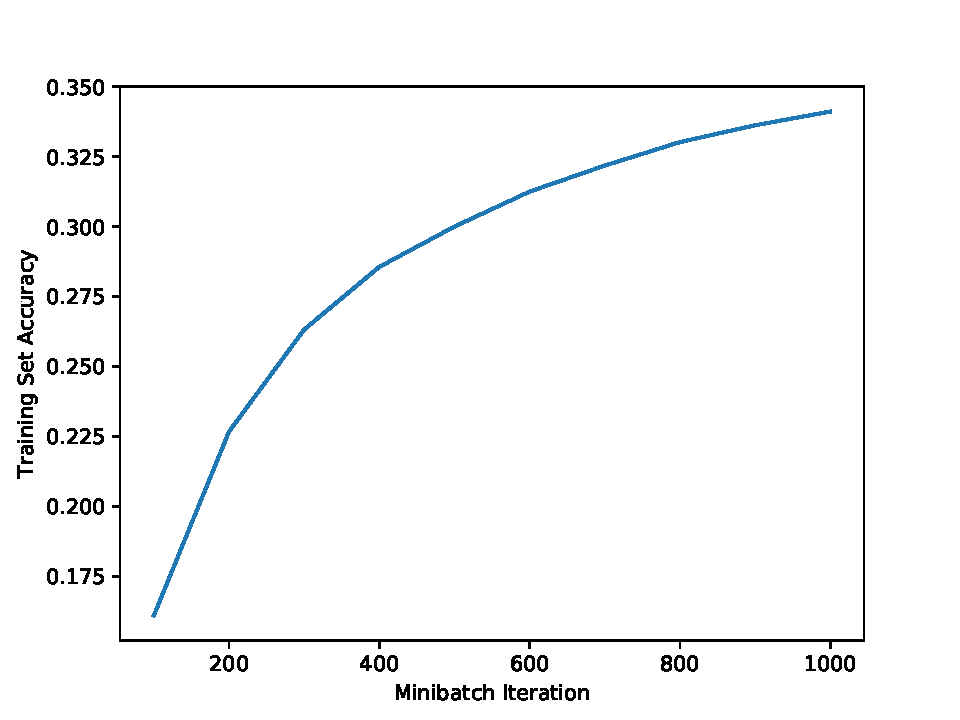
\includegraphics[width=\columnwidth]{img/accuracy}
\caption{
Classification accuracy on training data for our prototype network over 1000 256-example minibatch training iterations.
}
\label{fig:accuracy}
\end{figure}
\begin{figure}
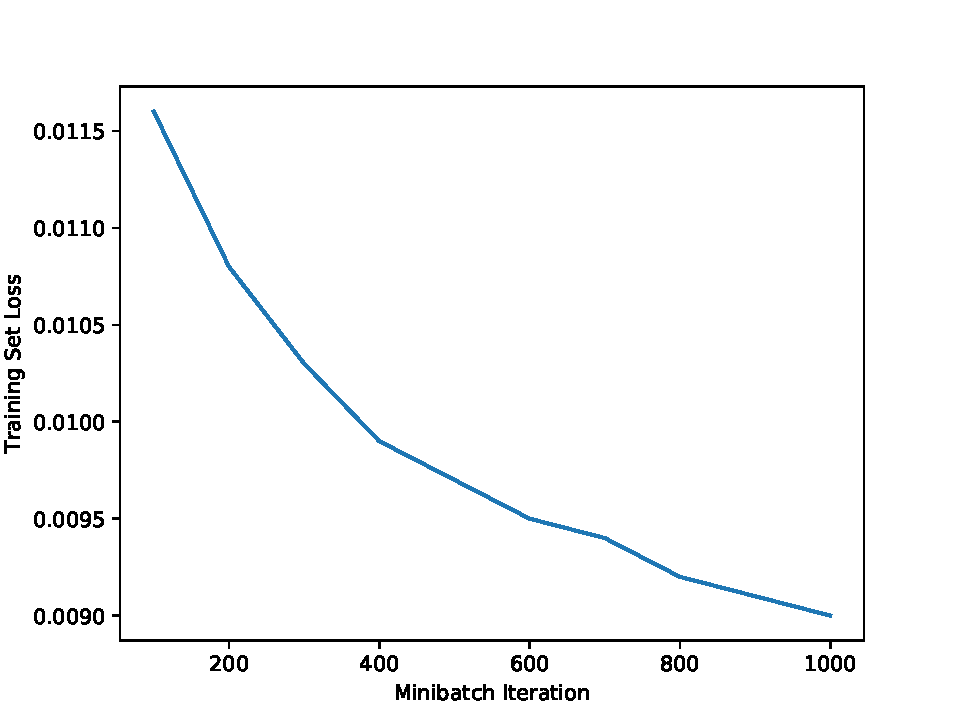
\includegraphics[width=\columnwidth]{img/loss}
\caption{
Cross entropy loss on training data for our prototype network over 1000 256-example minibatch training iterations.
}
\label{fig:loss}
\end{figure}

For our preliminary experiments, trained our model to differentiate between the 23 top-level categories that had more than 50,000 training examples.
As shown in Figures \ref{fig:accuracy} and \ref{fig:loss}, training data classification accuracy increased over the course of the training and training data cross entropy decreased over the course of the training process.
Training our prototype network with 5400 minibatches of 256 training examples, we achieved cross-entropy loss of 0.0080 and classification accuracy of 0.4020, both measured on training data.
As the cross-entropy loss and classification accuracies were measured using training data, these results should be taken with a grain of salt. 
Although less formal and less powerful than we ultimately hope to achieve, these results nonetheless demonstrate that our data wrangling and network training pipelines are in good working order.

The major constraining factor of our preliminary experiment was computational power.
Because of the model's size, training our model on 6400 examples takes approximately 20 minutes.
To preserve our Google credits, we kept the training of our prototype model to a minimum required in order to demonstrate that we have our data manipulation and training processes properly configured.   
 
\section{Milestones}
 

\textit{Midterm report --- November 12, 2017}

For our midterm report we have a working prototype solution for high level classifications and have preliminarily demonstrated the functionality of our model on high level classification.
\\


\textit{Final report --- December 13, 2017}

When we reach the final report, we hope to have a fully implemented model to organize products at all three levels of categorization.
We will work to resize the scale of the problem that we're tackling to our limited computational resources in a way that preserves its most important characteristics (i.e. many-class, hierarchical classification) while rendering it feasible to complete. 
We will use cross validation to assess and report the performance of our final model on image classification at all three hierarchical levels for a manageable subset of the available Cdiscount categories.
We will use different, larger, ResNet architectures, hopefully up to ResNet152. Furthermore, we will fine-tine these networks during training rather than simply use them as feature extractors for the image classification task. 
For the more multi-class versions of this problem, we may use a K-nearest neighbors approach to the final classification in place of softmax cross entropy. This will only be implemented if other approaches are deemed insufficient.

\section{Division of Labor}

For efficiency, we divided preliminary labor across different types of tasks that could be completed independently.
For the final project, we will collaborate more closely in person on the model building, training, and testing to ensure that all group members are hands-on with all aspects of our model. 

\textit{Steven}

Prepared data, ran statistical scripts on the data, and compiled high-level observations about the data. 

\textit{Matthew}

Created visualizations, compiled results, and completed the write up.

\textit{Ian}

Created dataset iterator and classification script (see Github). 

\section{Code}
Our code is available at:
\begin{itemize}
\item \textit{https://github.com/ianwhale/cse891}

This repository has scripts for dataset preparation and analysis, our dataset iterator, and our model design/training.
\item \textit{https://github.com/mmore500/cdiscount-datavis}

This repository has scripts for creating the data visualizations presented in this report.
\end{itemize}



{\small
\bibliographystyle{ieee}
\bibliography{egbib}
}

\end{document}
